\chapter{Preliminary Analysis of a Rocket}
The following chapter describes the functionality and structure behind a rocket. The goal is to determine which factors that leads to instability in flight and launch of a rocket. 



The full scale rocket model that will be described consist of,
\begin{itemize}[noitemsep]
\item a payload system.
\item a guidance system.
\item a propulsion system. 
\item a structural system.
\end{itemize}    
The model is seen cf. figure \ref{fig:RocketStructure}.
\begin{figure}[htbp]
	\centering
 	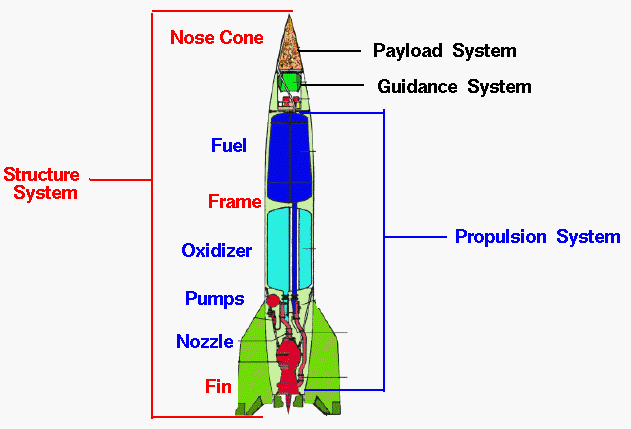
\includegraphics[width=0.65\textwidth]{figures/RocketStructure.png} 
 	\caption{Structure of a full scale rocket.}
 	\label{fig:RocketStructure}
\end{figure}
%https://spaceflightsystems.grc.nasa.gov/education/rocket/rockpart.html

\textbf{Payload System}\\
Most rockets has some form of a payload system. The goal of the payload system is to carry different objects to its wanted destination. The payload can be everything from satellites and astronauts to fireworks depending on the purpose of the rocket. 


\textbf{Guidance System}\\
All rockets that has the goal to be directed or controlled includes a guidance system. The guidance system consist of a processors, sensors, radars, and  a form of wireless communication. Its purpose is to control the stability, direction and rotation of the rocket during launch and in flight. The guidance system is developed based on the understanding of forces acting rocket and its motion. The guidance system in moderne rockets often actuate on the propulsion and nozzle system to correct rotation and direction of the rocket.

\textbf{Propulsion System}\\
The propulsion system of a rocket is the part which thrust the rocket. Thrust is the the main force that makes the rocket launch and fly. All propulsion systems is based on Newton's third law. This means that a propulsion system should be able make a combustion which produces a downwards force high enough to launch the structural system of the rocket.


The propulsion system can either be a liquid rocket engine or a solid rocket engine. A liquid rocket engine is based on a combustion of fuel and a oxidizer which is mixed an burned. The resulting gas of the burn, is directed trough a nozzle which accelerates it.
A solid rocket engine has premixed oxidizer and fuel which becomes the propellant. This propellant is compressed into a cylinder with an hole in it that functions as a combustion chamber. Which means that after ignition the propellants surface functions as the combustion chamber. The gas is therefore also forced trough a nozzle that accelerates it. Which applies i force to the engine that gives a launch of the rocket. 


\textbf{Structural System}\\
Close to all full scale rockets consist of a structural system. The system consist of the cylindrical body/frame, a nose cone with the payload system and the fins that ensures a stable aerodynamic profile. Though most newer full scales rocket does not rely only on aerodynamics to ensure stability.
\bigbreak   

The combinations of these 

%All based on https://spaceflightsystems.grc.nasa.gov/education/rocket/rockpart.html

\subsection{Controlling a Rocket's Stability}
The design method for placing the CP and GP does not always provide a perfectly stable attitude control. Indeed to have such precision an active control system is necessary. Full scale rockets use the thrusting force to achieve alike control. In order to do so most of them operate with the gimbaled thrust method. It consists of steering the engine's nozzle to get the thrusting force in right incidence. An example is seen cf. figure \autoref{fig:RocketGimbal}. 
\begin{figure} [htbp]
	\centering
	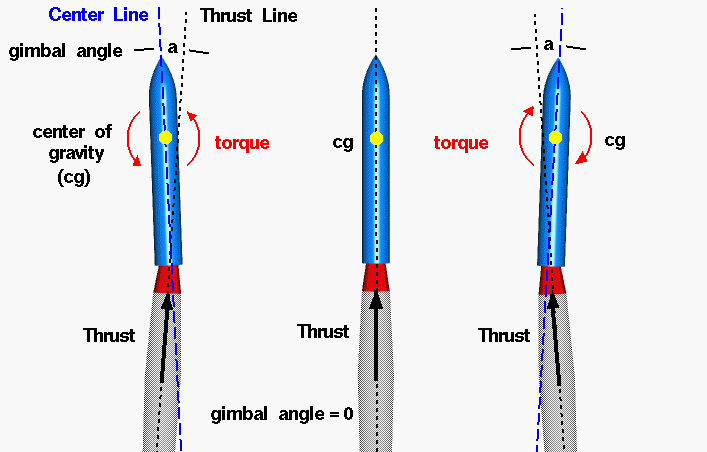
\includegraphics[width=0.8\linewidth]{RocketGimbal}
	\caption{Example of gimballing a rocket nozzle \cite{web:rocketnasa}.}
	\label{fig:RocketGimbal}
\end{figure}
\newpage

Where a torque is applied to create a rotation around the rocket's center of gravity. The thrust direction is relative to the position of the center of gravity.  This should compensate for direction deviations from the rocket's center line or trajectory, and keep the rocket stable. The described gimbal method will be the control method focused on in this project. The rocket will be designed with a control system depending on vectoring the thruster in relation to the attitude position of the rocket. 


\section{Mechanical System of a Rocket}
Input/output relation of a rocket.
\section{The Inverse Pendulum}
relate the rocket model to a Inverse Pendulum